%%
%% This file is modified from the ACM sigconf template.
%%
\documentclass[sigconf]{acmart}

\usepackage{graphicx}
\graphicspath{ {./images/} } 
%% Remove ACM Reference Format and citation information
\settopmatter{printacmref=false} % Removes citation information below abstract
\renewcommand\footnotetextcopyrightpermission[1]{} % Removes footnote with conference information in first column

\acmConference{CS 5805 Machine Learning} % Conference name
\acmYear{Fall 2024} % Year

\title{Facial Expression Recognition in Context of Driving}

%% Authors and affiliations
\author{Syed Talal Hasan}
\email{syedtalal@vt.edu}
\affiliation{%
  \institution{Virginia Polytechnic Institute and State University}
  \city{Blacksburg}
  \state{VA}
  \country{USA}
}

\author{Muhammad Hamza}
\email{muhamza@vt.edu}
\affiliation{%
  \institution{Virginia Polytechnic Institute and State University}
  \city{Blacksburg}
  \state{VA}
  \country{USA}
}

\author{Mughees Ur Rehman}
\email{mughees@vt.edu}
\affiliation{%
  \institution{Virginia Polytechnic Institute and State University}
  \city{Blacksburg}
  \state{VA}
  \country{USA}
}

\author{Yeana Lee Bond}
\email{yeana@vt.edu}
\affiliation{%
  \institution{Virginia Polytechnic Institute and State University}
  \city{Blacksburg}
  \state{VA}
  \country{USA}
}

%% Short author list for page headers
\renewcommand{\shortauthors}{Talal, Hamza, Mughees, Yeana Lee Bond}

\begin{document}

\begin{abstract}
Driving can be an essential part of daily life, and more than 80\% of the drivers in the US feel safer with Advanced Driver Assistance Systems (ADAS). It is foreseen that in-vehicle technologies such as ADAS leveraging the concept of Natural User Interface, which can incorporate Affective Computing using computer vision, will become integral components of intelligent driver assistance systems in the future. While human emotions are diverse and tricky especially in terms of how they are interpreted, we are curious how many images are needed for state-of-the-art machine learning models in computer vision to well classify three basic human emotions that could be triggered while manually driving: neutral, happy, and angry emotions. Our evaluation from comparing EfficientNet, Vision Transformer, and CNN-based models suggests that EfficienNet with just 4M parameters is the most effective model with the accuracy of 96\% if the number of images are more than 1000 considering its faster training time while Vision Transformer with 86M parameters achieves the accuracy of 87\% with 600 images after being fine-tuend on Multiple Light Intensities Driver Emotion Recognition (MLI-DER). Additionally, with comparing our custom CNN-based models with 9M parameters to the base model with 3M parameters, we learned that it is the architecture, not the number of parameters of the CNN-based models, that determine the model performance on our test dataset, MLI-DER. Lastly, we learned that our results reflect two fundamental insights in machine learning: the importance of dataset distribution and quality.


\end{abstract}

\keywords{Facial Expression Recognition, Facial Emotion Recognition, In-vehicle intelligent system, Maching Learning, Vision Transformer, EfficientNet, Transfer Learning, Hybrid Models, Deep Learning, Computer Vision}


\maketitle

\section{Introduction}
Driving can be an essential part of daily life \cite{10486424}, \cite{bengler2014three}, \cite{wang2021survey}, and more than 75\% of Americans believe that technologies can significantly improve road safety according to the Safer Mobility Survey carried out to gauge Americans' views on road safety for all road users in 2022 \cite{paveaeye2023}. This survey of 1,095 adults revealed that 78\% view technology as very or somewhat important in addressing driving safety concerns, while 82\% feel safer with Advanced Driver Assistance Systems (ADAS) in vehicles \cite{paveaeye2023}. 
\begin{figure}[h]
\caption{Based on Russell's Circumplex Model of Affect \cite{russell1980circumplex}, the neutral, happy, and angry emotions are indicated with blue circles\cite{kopalidis2024advances}}
\centering
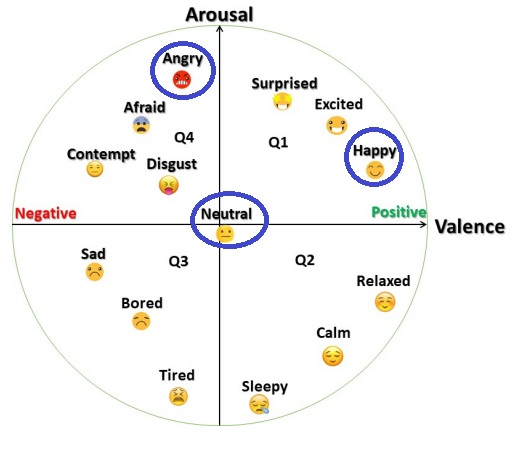
\includegraphics[width=9cm, height=7cm]{images/ml_figure1.jpg}
\end{figure}
Additionally, a research by the Insurance Institute for Highway Safety indicates that blind spot detection has contributed to a 14\% reduction in lane change crashes \cite{paveaeye2023}.

ADAS has evolved over several decades, with early iterations appearing in the mid-20th century \cite{bengler2014three}. One of the earliest examples is cruise control, invented in 1948 by Ralph Teetor, which allowed drivers to maintain a constant speed without manual acceleration \cite{motorCities2021}. In the 1950s, radar-based assistance systems were introduced in concept cars. For instance, Ford's FX-Atmos concept car featured radar technology to detect objects ahead, providing visual information to the driver \cite{fordSuper03}. Similarly, General Motors' 1959 Cadillac Cyclone showcased a radar-based braking assistance system \cite{motorCities2021}. 

With exteroperceptive sensors including cameras,  ADAS has become more intelligent in lane-keeping or lane-changing , pedestrian or object detection \cite{bengler2014three}, distance-keeping while also capturing driving styles or road conditions \cite{zepf2020driver}. As newer vehicles are equipped with advanced automation features, offering a broader range of driver assistance and autonomous capabilities \cite{navonchallenging}, \cite{sae2021j3016},   researchers in human factors and human-computer interaction have focused on detecting driver states discerning ways to reduce the factors derived from driver states such as emotions or fatigue \cite{10486424}, \cite{murali2022intelligent}. As a result, we can find that Suburu's Driver Monitoring System monitors signs of driver's sleepiness or inattention and also that BMW's Active Driving Assistant with Attention Assistant analyzes driving behavior and can advise the driver to rest \cite{10486424}. Yet, there have been relatively fewer examples that employ human emotions to improve safety in real world even though some empirical research results imply that emotions could be causes of distractions and inattention which may threat safety of the drivers and the road while driving \cite{chan2015emotion}, \cite{cunningham2016impact}. 

Generally speaking, human emotions are diverse and tricky especially in terms of how they are interpreted which may vary depending on cultural and/or situational contexts \cite{izard2013human}, \cite{picard2003affective}, \cite{kang2019extracting}. While it is not only computer vision techniques, but also other approaches using other physiological data such as heart rate, electroencephalogram signals from brain, or electrical conductance across skin could contribute to accurately analyzing emotions \cite{pidgeon2022end}, \cite{shu2018review} we are interested in labeling emotions into three classifications, neutral, happy, and angry emotions as shown in Figure 1 with a question of how many samples are needed to achieve an acceptable accuracy by taking the approach of "Facial Emotion Recognition" or "Facial Expression Recognition" \cite{ekman1992facial} both which are abbreviated as "FER." 

Many machine learning and computer vision frameworks train models on labeled data that do not clearly differentiate between facial expressions and emotions \cite{kopalidis2024advances}. This implies that "FER" refers to the algorithms that detect these observable expressions, without making any claims about the psychologically true emotional states behind them . Thus, in this present work, we adopt the term "Facial Expression Recognition (FER)" as it reflects the detection of observable, physical expressions, recognizing that a facial expression can be triggered by an underlying emotion or emotional state.

It is important to note, however, that when we classify facial expressions, we use the term "emotion," implying that a detected facial expression is assumed to have been triggered by a corresponding emotion. This assumption persists despite our inability to ascertain the true internal psychological state of the person captured in a two-dimensional image. The distinction between observed expression and actual emotional experience remains a challenge, as beyond facial cues alone in reality, emotions are complex and influenced by various factors.

Just as Automatic Emergency Braking is becoming mandatory in new vehicles across various regions of the world \cite{bengler2014three}, the ability to detect and respond to a driver's emotional states may also become a required feature in future vehicles. Nowadays, vehicles are manufactured with higher levels of driving automation. This means that drivers will have more time to interact with advanced an in-vehicle Natural User Interface (NUI) \cite{murali2022intelligent}. This interface will likely incorporate the ability to engage in verbal conversations with drivers, creating a more human-like interaction experience. Such a system could also reflect and respond to human emotions expressed both verbally or facially, providing personalized suggestions or recommendations for actions, entertainment, or rest, ultimately enhancing driver satisfaction and road safety \cite{murali2022intelligent}.

Detecting human expressions, including facial expressions, can play a critical role in analyzing drivers' emotional states to enhance safety and the overall driving experience \cite{murali2022intelligent}, \cite{zepf2020driver}. By interpreting these expressions in real-time, such systems can detect critical conditions—such as fatigue, distraction, or stress—and facilitate proactive interventions to help prevent accidents \cite{murali2022intelligent}. Future in-vehicle technologies are expected to leverage NUI and Affective Computing \cite{picard2003affective}, powered by computer vision \cite{kang2019extracting}, as integral components of intelligent driver assistance systems. This motivates our exploration of how current state-of-the-art machine learning algorithms can effectively label three fundamental human emotions from images of facial expressions within the context of manual driving.


The remainder of this paper is organized as follows: Section 2 provides an overview of related work and approaches commonly adopted by Facial Expression Recognition researchers. Sections 3 and 4 detail the selected machine learning models used for analysis and comparison, including our custom Convolutional Neural Network (CNN) models with two distinct parameter configurations. Section 5 presents the findings from our comparison of these models. Section 6 reports first fine-tuning results and our final conclusion based on our comparison results and evaluation. In Section 7, we discuss insights we gained from our experiment in comparing CNN-based models with different numbers of parameters and share fundamental insights reflected in our comparison results. Finally, Section 8 outlines potential directions for future work.



\section{Related Work}

Facial Expression Recognition (FER) research has undergone significant evolution, transitioning from handcrafted techniques to advanced deep learning models \cite{kopalidis2024advances}. Early FER methods relied on handcrafted features such as Histograms of Oriented Gradients (HOG), Local Binary Patterns (LBP), and Gabor filters \cite{kopalidis2024advances}. These methods used geometric and appearance-based features to classify facial expressions via traditional classifiers like Support Vector Machines (SVMs) and Hidden Markov Models (HMMs) \cite{kopalidis2024advances}. For example, a study introduced a Weighted Random Forest (WRF) classifier optimized for real-time, low-resource environments \cite{jeong2018}. This approach achieved competitive performance on datasets like CK+ and MMI Facial Expression Database, but the reliance on hand-crafted features made these methods vulnerable to real-world challenges, such as occlusions, lighting variations, and pose changes \cite{kopalidis2024advances}.

The rise of deep learning marked a transformative phase in FER research. Convolutional Neural Networks (CNNs) revolutionized the field by automatically learning hierarchical and discriminative features directly from image data \cite{kopalidis2024advances}. EfficientNet, a model proposed for scaling neural networks efficiently, achieved state-of-the-art performance with fewer computational resources \cite{tan2019}. A follow-up study demonstrated the effectiveness of fine-tuning pre-trained EfficientNet models on data-scarce FER scenarios, such as CK+ and JAFFE datasets \cite{lyons1998japanese}, showcasing its adaptability and efficiency \cite{alam2022}.

Building on the success of deep learning, Vision Transformers (ViTs) have recently been applied to FER tasks \cite{dosovitskiy2020image}. Unlike CNNs, ViTs use a self-attention mechanism that excels in capturing global spatial relationships within images, making them well-suited for analyzing complex patterns in facial expressions \cite{dosovitskiy2020image}, \cite{kopalidis2024advances}. One study fine-tuned ViTs on the JAFFE dataset, which contains facial expressions from Japanese female subjects categorized into six basic emotions and neutral expressions, achieving 96.06\% accuracy \cite{febrian2024}. Another study applied ViTs to AffectNet \cite{8013713}, a larger and more diverse dataset of facial expressions, achieving an accuracy of 64.48\% \cite{roka2023}. These results demonstrate ViTs' capabilities but also highlight their reliance on large datasets, which limits their applicability in data-scarce environments.

To address these limitations, hybrid models have emerged that integrate traditional and modern approaches. For instance, a study combined LBP features with CNN-based representations, using attention mechanisms to emphasize critical facial regions \cite{ma2021}. This hybrid approach achieved robust performance on challenging datasets like RAF-DB \cite{li2017reliable}, FERPlus \cite{barsoum2016training}, and AffectNet \cite{8013713}, demonstrating its ability to handle occlusions and pose variations effectively.

Transfer learning has also proven to be a critical strategy for overcoming data scarcity. Fine-tuning pre-trained EfficientNet models on small datasets like CK+ and JAFFE significantly improved accuracy while maintaining computational efficiency, underscoring the value of transfer learning in enabling high performance with limited resources \cite{alam2022}.

The evolution of FER can be summarized as follows: (1) early approaches relied on handcrafted features and traditional classifiers but faced limitations in real-world scenarios; (2) CNNs revolutionized FER with automated feature learning and superior performance on constrained datasets; (3) Vision Transformers extended FER capabilities by capturing global spatial relationships, although they depend on large datasets; (4) hybrid models bridged the gap between traditional and deep learning approaches, enhancing robustness; and (5) transfer learning emerged as a solution for data-scarce environments. Today, FER research emphasizes hybrid models and transfer learning to balance efficiency, scalability, and robustness. However, challenges such as cultural variability, scalability, and real-world deployment persist, requiring further exploration in future research \cite{jeong2018, tan2019, alam2022, febrian2024, ma2021, roka2023, kopalidis2024advances}.


\section{Methodology}

The overaching goal of our project is to evaluate and compare the performance of three machine learning models—EfficientNet \cite{tan2019}, Vision Transformer (ViT) \cite{dosovitskiy2020image}, and a Convolutional Neural Network (CNN)—on the task of emotion recognition \cite{kopalidis2024advances}. We employed the FER-2013 dataset \cite{fer2013kaggle}, a widely-used benchmark dataset for facial emotion recognition, as our base dataset. The FER-2013 dataset contains images depicting a range of emotions (e.g., happiness, sadness, anger, surprise, etc.) \cite{fer2013kaggle}, which we used to initially train and assess the three models.

The first step of the analysis involved training the three selected models on the FER-2013 dataset using their respective architectures and hyperparameter settings. EfficientNet and the CNN-based modles were each trained for 50 epochs, while the Vision Transformer was trained for 5 epochs due to its computational complexity and sensitivity to training time. After this initial training phase, we observed that the achieved accuracies across all models were suboptimal, which prompted us to consider fine-tuning the models to improve performance.

To investigate the effect of training data size on model performance, we fine-tuned each model using subsets of a primary  dataset, MLI-DER. This fine-tuning process involved progressively increasing the number of training samples to determine the optimal size to achieve higher accuracy. The subsets of the MLI-DER dataset were incrementally increased in steps of 100 samples, starting from 100 up to 800 samples. At each step, the models were re-trained and validated, and their accuracy was recorded. This systematic approach allowed us to analyze the relationship between the training sample size and each model's performance, providing some findings into the models' capacity to learn from limited data.

\section{Model Comparison}

To compare the selected models comprehensively, we considered both their advantages and disadvantages based on performance, computational efficiency, and training behavior. Table \ref{tab:classifiers} provides a summary of key attributes, including model parameters and their respective performance on benchmarks such as CIFAR-100, where applicable.

\begin{table}[h]
  \caption{Comparison of Classifiers}
  \label{tab:classifiers}
  \centering
  \begin{tabular}{|c|c|c|c|}
    \hline
    \textbf{Attributes} & \textbf{Model} & \textbf{Params} & \textbf{CIFAR-100} \\
    \hline
    Lightweight & EfficientNet & 4 Million & 91.7\% \\
    \hline
    Accurate & Vision Transformer & 86 Million & 94.6\% \\
    \hline
    Simple & CNN-b1 & 3 Million & - \\
    \hline
  \end{tabular}
\end{table}


\subsection{EfficientNet}

EfficientNet is a highly optimized convolutional neural network that achieves the state-of-the-art performance through a combination of model scaling and architectural improvements \cite{tan2019}. It builds upon MobileNetV2 \cite{sandler2018mobilenetv2} as its foundation, utilizing inverted residual blocks and depth-wise separable convolutions to improve efficiency \cite{tan2019}. Depth-wise convolutions reduce the computational cost by performing spatial convolutions independently for each input channel, while the inverted residual blocks help maintain information flow even in deeper layers \cite{tan2019}. These architectural enhancements allow EfficientNet to achieve better accuracy with fewer parameters compared to traditional CNNs \cite{kopalidis2024advances}.

In our experiments, EfficientNet was trained for 50 epochs and demonstrated moderate performance improvements as the training sample size increased. Its key advantage lies in its computational efficiency, enabling high accuracy without the need for excessive parameters. Additionally, EfficientNet's ability to generalize well on limited data was evident during the process of fine-tuning. However, its reliance on pretraining and fine-tuning remains a notable drawback, as the model struggled to perform well when trained solely on the FER-2013 dataset without additional data. Despite this limitation, EfficientNet outperformed the baseline, the CNN-based model, demonstrating its superior feature extraction and scalability capabilities.

\subsection{Vision Transformer}
The Vision Transformer (ViT) introduces a fundamentally different approach to computer vision tasks by leveraging the self-attention mechanism, a concept originally designed for natural language processing \cite{dosovitskiy2020image}, \cite{kopalidis2024advances}. Unlike traditional CNNs that rely on convolutional filters to capture local spatial features, ViT can capture both local and global dependencies across an image, making it particularly powerful for tasks requiring subtle and interdependent feature recognition, such as facial emotion recognition \cite{dosovitskiy2020image}, \cite{kopalidis2024advances}.

The self-attention mechanism allows the model to identify which parts of the image are most important to make a classification and relate different regions to each other \cite{dosovitskiy2020image}. For example, in facial expression recognition, the model can learn to connect the squinting of the eyes with the smile of the mouth, understanding that these features together are indicative of happiness. This ability to establish relationships between distant parts of the image enables ViT to better understand the overall context of an emotion rather than focusing on isolated features \cite{dosovitskiy2020image}.

During training, ViT divides the input image into fixed-size patches, flattens them, and embeds them into a sequence of tokens \cite{dosovitskiy2020image}. These tokens are then passed through multiple layers of self-attention, where each token "attends" to all other tokens in the image \cite{dosovitskiy2020image}. This global attention mechanism ensures that the model considers every patch in the image when determining its relevance, allowing ViT to recognize nuanced patterns and relationships that might be missed by convolutional approaches \cite{dosovitskiy2020image}.

In our experiments, the ViT was trained for 5 epochs, and despite the shorter training duration, it demonstrated promising performance as the training sample size increased. This highlights its ability to generalize effectively even when data is limited. However, ViT's reliance on larger datasets for full optimization remains a challenge, as its performance can degrade if insufficient training data are available. Additionally, its computational demands are significantly higher compared to EfficientNet or CNN-based models. Nevertheless, ViT’s self-attention mechanism proved to be a significant advantage in capturing global context, making it well-suited for emotion recognition tasks that require understanding complex facial expressions.

\subsection{Convolutional Neural Network}
The CNN model we initially employed had a relatively small architecture with 3 million parameters. During the initial training phase, this model performed poorly, achieving the accuracy of only 33\%. Given this low performance, we hypothesized that the issue might stem from the simplicity of the network architecture, which could limit its capacity to extract complex features necessary for accurate emotion recognition. To address this, we increased the size of the CNN model to a larger architecture with 9 million parameters, aiming to improve its representational power and overall accuracy.

However, despite the increased model size, the CNN-based model continued to underperform relative to the other models. This suggested that simply scaling the architecture did not resolve the underlying issues, possibly due to factors such as insufficient training data, suboptimal feature extraction, or overfitting on the limited dataset sizes. The CNN's poor results underscored its limitations in handling the complexity of facial emotion recognition, especially when compared to more advanced architectures like EfficientNet and Vision Transformer.

\section{Findings}



After fine-tuning EfficientNet B0 and Vision Transformer on the FER-2013 dataset and training a custom CNN-based model from scratch, we evaluated their performance on the FER-2013's test set, which consists of over 3,000 images evenly distributed among the three classes. Among the models, Vision Transformer achieved the highest accuracy at 88\%, followed by EfficientNet B0 at 79\%, and our custom CNN architecture at 70\% as shown in Table 2.

\begin{table}[h]
  \caption{Model Performance: FER-2013}
  \label{tab:fer2013-performance}
  \centering
  \begin{tabular}{|c|c|c|}
    \hline
    \textbf{Model} & \textbf{Parameters} & \textbf{Test Accuracy (\%)} \\
    \hline
    EfficientNet & 4M & 79 \\
    \hline
    Vision Transformer & 86M & 88 \\
    \hline
    CNN-b1 & 3M & 70 \\
    \hline
  \end{tabular}
\end{table}

These results aligned with our expectations, as the state-of-the-art accuracy for the full FER-2013 dataset stands at 76\% using Vision Transformer, while CNN-based approaches typically face challenges in achieving comparable performance. These findings supported our hypothesis that Vision Transformer would outperform the other models on the FER-2013 dataset.
When we evaluated the models without fine-tuning on the Multiple Light Intensities Driver Emotion Recognition (MLI-DER) dataset \cite{10226464} to assess their generalization capabilities, we found that none of them performed well. All the models achieved an accuracy of approximately 30\%, indicating that they were effectively guessing randomly for the 3-class classification task. This result aligned with our hypothesis, as the MLI-DER dataset includes not only the faces of individuals but also their entire bodies, backgrounds, and chairs, which differ significantly from the face-only images in the FER-2013 dataset. While we had anticipated the Vision Transformer model to perform better due to its ability to extract context from image patches, it also failed to surpass random guessing, highlighting the importance of domain-specific fine-tuning for effective generalization.

After observing that the models did not generalize to the MLI-DER dataset when trained solely on FER-2013, we aimed to determine the minimum number of samples required to fine-tune each model to achieve an accuracy of over 80\%. We set this benchmark based on the performance of Vision Transformer on the FER-2013 dataset, where it achieved the highest accuracy of 88\%, while our custom architecture and EfficientNet remained around 70\% as compared in Table 3.
\begin{table}[h]
  \caption{Model Performance: MLI-DER}
  \label{tab:mli-der-performance}
  \centering
  \begin{tabular}{|c|c|c|c|}
    \hline
    \textbf{Model} & \textbf{Params} & \textbf{Accuracy (\%)} & \textbf{F1 Score} \\
    \hline
    EfficientNet & 4M & 82 & 0.82 \\
    \hline
    Vision Transformer & 86M & 87 & 0.85 \\
    \hline
    CNN-b1 & 3M & 33 & 0.31 \\
    \hline
    CNN-b2 & 9M & 32 & 0.31 \\
    \hline
  \end{tabular}
\end{table} 

Additionally, we became interested in fine-tuning the models for fewer epochs than initially trained and using a very small subsample of the MLI-DER dataset. The goal was to assess the models' performance on a much larger test set of approximately 1,000 images. Once again, the Vision Transformer outperformed the other models, achieving the accuracy of 87\%, followed by EfficientNet with 82\%. This comparison result further proved that the Vision Transformer's superior ability to adapt with minimal fine-tuning.

What was particularly surprising was that our custom CNN-based architecture failed to fine-tune entirely. With the CNN-based model with 3M parameters, its accuracy remained at 33\% throughout the fine-tuning process, regardless of the sample size used. We hypothesized that this behavior could be attributed to the limited number of parameters in the model, as it is significantly simpler compared to the other two architectures. To test this, we constructed a fourth model following the same CNN + dense layer principle but with 9 million parameters, a substantial increase compared to the original architecture. However, even this modified architecture failed to fine-tune and remained stuck at approximately 32\% accuracy, suggesting that the lack of fine-tuning was not solely due to the parameter count. Among the three architectures, Vision Transformer stood out, achieving the best performance with an F1-score of 0.85 and the highest accuracy. This further demonstrated its robustness and adaptability compared to the simpler CNN-based models.
Both EfficientNet and Vision Transformer demonstrated superior robustness and adaptability compared to the simpler CNN-based models, successfully surpassing the 80\% accuracy threshold we had set. VisionTransformer achieved this threshold with just 600 samples, while EfficientNet required 800 samples to cross the mark. 

\begin{figure}[h]
\caption{Each model's Test Accuracy with different number of parameters and different number of samples on MLI-DER}
\centering
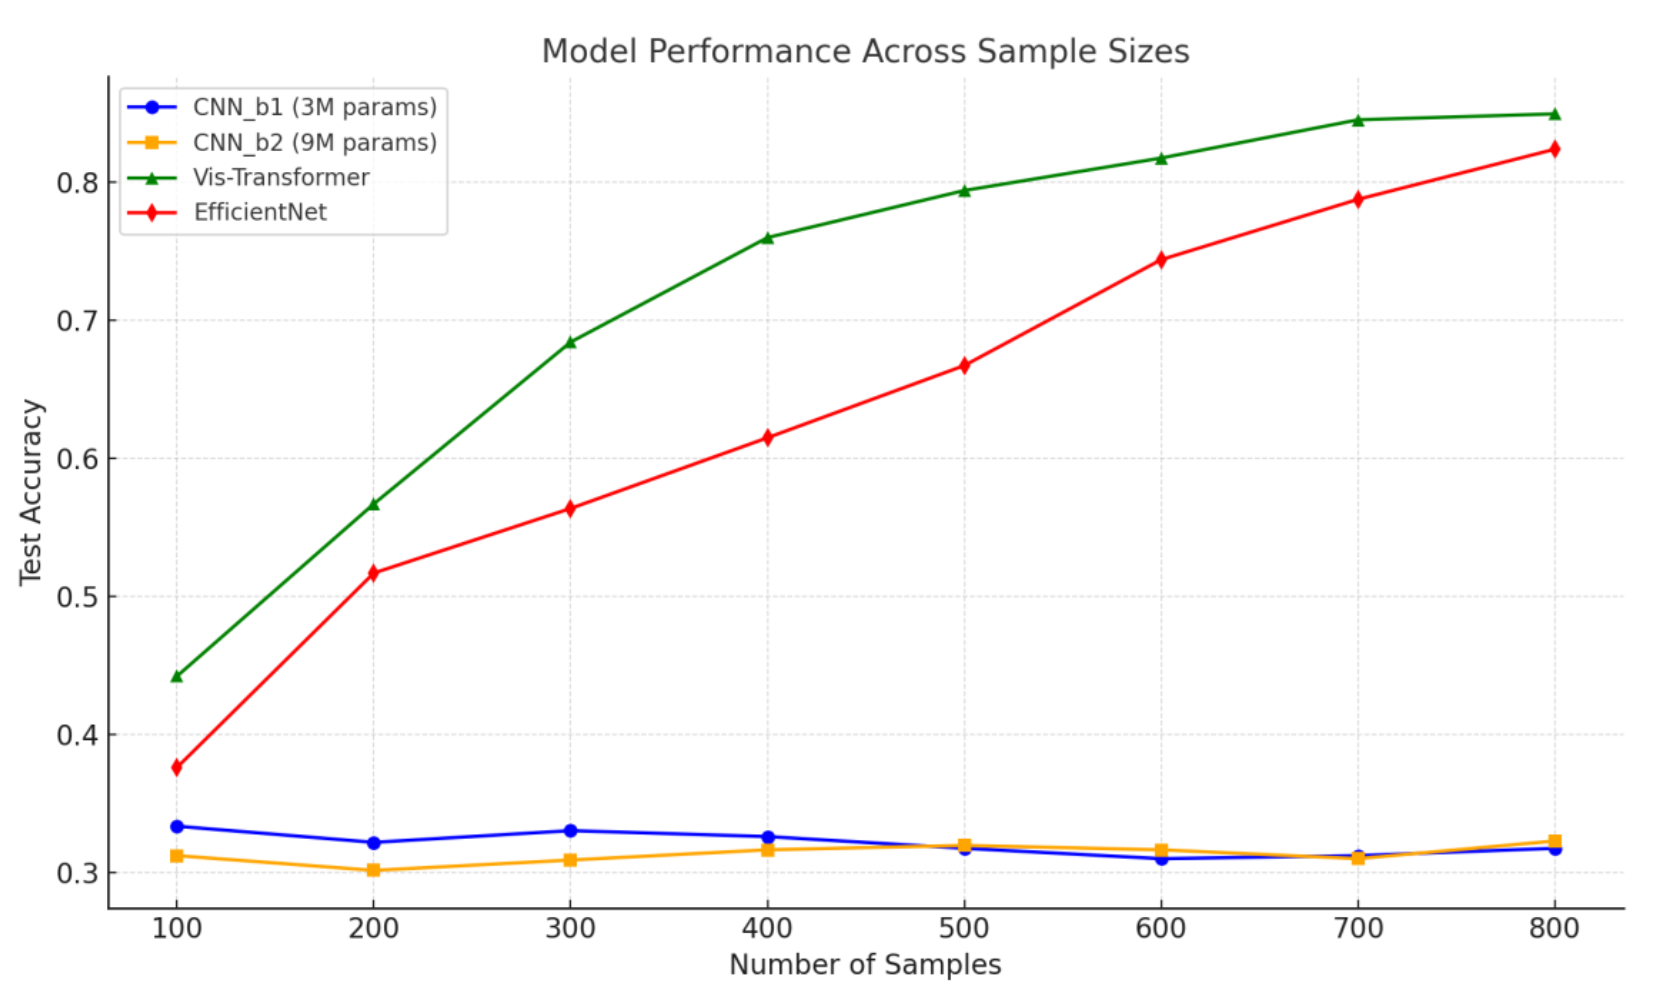
\includegraphics[width=9cm, height=7cm]{performance}
\end{figure}

Analyzing the relationship between sample size and accuracy revealed an interesting trend as depicted in Figure 2: the graph for Vision Transformer displayed an elbow point at around 600 samples, suggesting diminishing returns with additional data beyond this point. In contrast, the graph of EfficientNet maintained a linear trend, indicating steady improvements as the sample size increased.

Given EfficientNet's faster training time, we conducted an additional experiment to explore its performance ceiling and determine if it could surpass 90\% accuracy. By fine-tuning the EfficientNet model with over 1200 samples for 30 epochs, we achieved an impressive accuracy of 96\%. This experiment revealed two key findings. First, the MLI-DER dataset appears to have more easily extractable semantic information compared to the FER-2013 dataset, enabling higher accuracy with sufficient samples. Second, having over 1000 samples is an optimal dataset size for EfficientNet when the accuracy threshold is set at 90\% or higher.




\section{Conclusion}

In this present study, we compared three state-of-the-art models—VisionTransformer, EfficientNet, and custom CNN-based models with two parameter configurations (3M and 9M)—to evaluate their performance of recognizing facial expressions in the context of manual driving using FER-2013 and MLI-DER datasets. We learn that it is the CNN-based model's architecture, not the number of parameters because the accuracy of our custom CNN-based models with either of 3M or 9M parameters stay at 31 - 32\% accuracy with the same F1 Score, 0.31. Our findings from our comparing work of EfficientNet with 4M parameters and Vision Transformer with 86M unveil EfficientNet's potential as a highly efficient and accurate model for facial expression recognition. By fine-tuning the EfficientNet model on the MLI-DER dataset with over 1200 samples for 30 epochs, we achieved an impressive accuracy of 96\% while with the sample of 600 while achieving an acceptable accuracy higher than 80\% with Vision Transformer model. Considering the difference in the number of parameters, this result implies that EfficientNet's scalability with sufficient training data and confirms that approximately, 1000+ samples is an optimal dataset size using the MLI-DER dataset in order to achieve a high accuracy with the model.


\section{Discussion}
Based on our results, we dived deeper into the MLI-DER dataset and discovered that most of the images in a single class were very similar. Since this is a driver facial emotion dataset with multiple light intensities, and it has a small number of drivers, the emotions of the same driver are repeated over time. Furthermore, since the drivers are from a single ethnicity, this dataset would not translate well to human facial expressions of other ethnicities, communities and/or nationalities. Therefore, our analysis reflects two fundamental insights in machine learning: The importance of dataset distribution and quality. We found out that with repeated emotions and single ethnicity of the MLI-DER dataset, the fine-tuned models on FER-2013 does not perform well. This finding underscores the principle that data matters—test and training datasets should share the same distribution—and data quality matters, as semantically rich datasets significantly enhance model learning.

\section{Future Work}

For future work, more diverse, unbiased datasets for broader applicability could be used according to the insights and key findings we gained. 
Applying face restoration techniques, such as Codeformer \cite{zhou2022towards}, and upscaling methods such as Enhanced super-resolution generative adversarial network (ESRGAN) \cite{wang2018esrgan} to the FER-2013 dataset could significantly enhance the dataset's utility. The FER-2013 dataset is known for its relatively low resolution, which can hinder the model's ability to extract fine-grained facial features, particularly in subtle expressions or microexpressions \cite{pfister2011recognising}.

Codeformer restores degraded facial details by reconstructing sharper and more semantically accurate features \cite{zhou2022towards}, while ESRGAN upscales images to a higher resolution, preserving essential textures and patterns \cite{wang2018esrgan}. By applying these techniques, we could provide a model with higher-quality input, enabling it to learn more effectively from nuanced facial features and achieve better performance. 

Another important improvement to this approach could be to use a larger facial emotion recognition dataset such as the AffectNet dataset \cite{8013713} that has about 0.4 million manually annotated images with valence and arousal information. This dataset is superior to FER-2013 and can lead to better generalization for the task of facial emotion recognition. Future works can look into using this dataset in conjunction with the MLI-DER dataset to improve the performance of the model. High-resolution data also helps reduce model overfitting on poor-quality images and allows for more precise feature extraction during training \cite{tian2011facial}.

Lastly, leveraging image embeddings and clustering to generate dataset labels offers an efficient alternative to manual annotation, which is time-consuming and prone to human error. Image embeddings represent facial images as feature vectors in a high-dimensional space, capturing meaningful relationships between similar expressions \cite{zhang2021learning}. Clustering algorithms, such as k-means or Density‐Based Spatial Clustering of Applications with Noise \cite{kremers2023two}, can group these embeddings based on their inherent similarities, automatically identifying patterns in the data \cite{vu2019efficient}. This approach may not only accelerate the labeling process but also enhance consistency and accuracy by removing subjective biases from manual labeling. Additionally, such methods may allow researchers to identify underrepresented classes in the dataset and facilitate the generation of pseudo-labels, which can then be refined through weak  supervision or active learning techniques \cite{vu2019efficient}. Thus, this approach may ultimately lead to results in a more balanced and representative dataset, further improving model training outcomes.



\nocite{*}
\bibliographystyle{ACM-Reference-Format}
\bibliography{references.bib}


\section{Statement of Work}

The contributions of each group member to this project are outlined below. Each member was responsible for specific sections of the project, with their roles and contributions detailed in Table~\ref{tab:statement-of-work}.


\begin{table*}[h]
  \caption{Statement of Work}
  \label{tab:statement-of-work}
  \centering
  \begin{tabular}{|c|p{12cm}|}
    \hline
    \textbf{Group Member} & \textbf{Contribution} \\
    \hline
    Syed Talal Hasan & Conducted the literature review by analyzing related works and summarizing key findings. Worked on data preprocessing, including cleaning and formatting the datasets (FER-2013 and MLI-DER) for model training. Processed and sampled the dataset to create the FER and MLI-DER dataset, designed and trained the custom CNN architectures and created the fine-tuning pipelines for the different architectures.  \\
    \hline
    Muhammad Hamza & Focused on the implementation and fine-tuning of Vision Transformers for the FER tasks. Worked on optimizing hyperparameters and analyzing the performance of transformer-based models on both datasets. \\
    \hline
    Mughees Ur Rehmaan & Contributed in training the EfficientNet model and evaluating its performance alongside other architectures. Designed visualizations and computed metrics to compare results across models. Additionally, developed a website to showcase project outcomes and participated in presentation discussions. \\
    \hline
    Yeana Lee Bond & Managed the training of models, ensuring proper configurations for training loops and validation while being on charge with finding datasets. Helped with data processing and explored EfficientNet's version 2. Took the lead on report writing, compiling the final document, and ensuring consistency in formatting and structure including all references. \\
    \hline
  \end{tabular}
\end{table*}




\end{document}
